% This is samplepaper.tex, a sample chapter demonstrating the
% LLNCS macro package for Springer Computer Science proceedings;
% Version 2.20 of 2017/10/04
%
\documentclass[runningheads]{llncs}
%\documentclass[runningheads]{article}
%
\usepackage[portuguese]{babel}
\usepackage{graphicx}
\usepackage{float}
\usepackage{booktabs}
\usepackage{minted}
\usepackage{xcolor}
% Used for displaying a sample figure. If possible, figure files should
% be included in EPS format.
%
% If you use the hyperref package, please uncomment the following line
% to display URLs in blue roman font according to Springer's eBook style:
% \renewcommand\UrlFont{\color{blue}\rmfamily}

\begin{document}
%
\title{Postgres Load Balancing Benchmark}
%
%\titlerunning{Abbreviated paper title}
% If the paper title is too long for the running head, you can set
% an abbreviated paper title here
%
\author{
Grupo 5 \\
Filipe Inês, n78775, º \\
Pedro Mendes, n97144, pedromendesfc@tecnico.ulisboa.pt
}
\authorrunning{Filipe Inês, Pedro Mendes}

\institute{Instituto Superior Técnico, Taguspark, Portugal}
%
\maketitle              % typeset the header of the contribution
%
\begin{abstract}
Um distribuidor de carga pode ser usado em bases de dados para oferecer alta disponibilidade e ganho de performance em pedidos de leitura apenas. Este projecto visa analisar a escalabilidade de uma base de dados PostgreSQL com o PGpool-II como distribuidor de carga. Como ferramenta de \textit{benchmark} utilizou-se a ferramenta PGbench. Observando os resultados obtidos é possível concluir que a instalação do PGpool num \textit{cluster} de bases de dados só será benéfica caso este seja alvo, maioritariamente, de transacções de leitura, caso contrário deverá ser dada atenção ao deterioramento da performance das transacções de escrita, tentando procurar soluções para mitigar este problema.

\keywords{Postgres  \and Scalability \and Pgpool \and Benchmark \and Pgbench.}
\end{abstract}
%
%
%
\section{Parte 1}

\subsection{Introdução}
O \textit{paper} escolhido~\cite{paper} explora a comparação de duas implementações distintas de distribuidores de carga para dois sistemas de base de dados conhecidos, MySQL e PostgreSQL. Porém, como o objectivo deste projecto era apenas analisar a escalabilidade de um sistema que respeitasse um conjunto de requisitos indicados num curto espaço de tempo e dado que o Postgres é um sistema robusto em produção, decidiu-se então focar a análise apenas no caso do PostgreSQL. 

A escolha do \textit{paper} deve-se à constante necessidade de sistemas de base de dados, nos dias de hoje, e como tal de que estes se mantenham eficientes e rápidos com o aumento da carga, fazendo com que, neste caso, a replicação e os distribuidores de carga ajudem nesse sentido. Assim, é necessário verificar a escalabilidade de tais sistemas ao introduzir réplicas e/ou distribuidores de carga.

\subsection{Âmbito}

Este projecto \footnote{Repositório Git - https://github.com/Mendess2526/ESLE-Postgres/releases/tag/1.0} foi desenvolvido no âmbito da unidade curricular de Engenharia de Sistemas de Larga Escala do Instituto Superior Técnico (Taguspark).

\subsection{Objectivo}

O projecto teve como objectivo analisar a escalabilidade de uma base de dados PostgreSQL ao adicionar réplicas da mesma e o distribuidor de carga PGpool-II. Para além disso, destinou-se também à utilização dos conceitos apresentados nas aulas teóricas da unidade curricular.

\subsection{Descrição do sistema}
PGpool-II é um \textit{middleware} posicionado entre os servidores PostgreSQL e clientes, actuando como cliente para os servidores e como servidor para os clientes. Este \textit{middleware} tem várias funcionalidades que incluem balanceador de carga, replicador de base de dados (para backups e robustez contra falhas), gestor de ligações e sistema de cache para \textit{queries}. 

Em geral o PGpool-II coordena um \textit{cluster} de base de dados tendo o porto e o \textit{hostname} de cada uma destas, este \textit{cluster} é formado por um \textit{master} e múltiplos \textit{slaves}. O \textit{master} pode receber transacções do PGpool-II de ambos os tipos (leitura e escrita), enquanto que os \textit{slaves} apenas recebem as transacções de escrita do \textit{master} e as de leitura do PGpool-II.
No \textit{cluster} a base de dados é replicada entre todos os \textit{slaves} podendo haver uma distribuição de transacções de leitura por entre os \textit{slaves}. \\

No âmbito deste trabalho vamos analisar o PGpool-II como balanceador de carga. É necessário notar que este \textit{middleware} apenas tem vantagens de escalonamento apenas sobre transacções de leitura e não a nível de transacções de escrita. Através da figura~\ref{fig:esquema} é possível observar o esquema genérico do sistema e a distribuição dos tipos de transacções.

\begin{figure}
    \centering
    \includegraphics[width=\textwidth]{images/pgpool_system.png}
    \caption{Esquema genérico da ligação entre cliente e servidor PostgreSQL.}
    \label{fig:esquema}
\end{figure}

\subsection{Workload}

O \textit{wordload} foi feito usando a ferramenta PGbench, esta baseia-se no TPC-B \textit{benchmark}\footnote{http://www.tpc.org/tpcb/}. Este pode ser visto como um \textit{stress test} de bases de dados, caracterizado por:

\begin{itemize}
    \item Quantidades significativas de I/O de disco
    \item Tempo moderado de execução do sistema
    \item Integridade das transacções
\end{itemize}

Cada transacção gerada pelo \textit{benchmark} contém cinco operações \textit{SELECT}, \textit{UPDATE} e \textit{INSERT} a não ser que seja seleccionado o modo apenas para leituras em que são feitos apenas operações \textit{SELECT}. Foram realizados testes, com duração de 60 segundos, de escritas e leituras para 1, 5, 10, 15, 20, 25 e 30 clientes em simultâneo para analisar \textit{clusters} com 0, 1, 2 e 3 \textit{slaves}. Os testes foram realizados com uma utilização máxima de 5\% do cpu por cada réplica.\par

% Quero o "porquê", o objectivo da cadeira é entender o sistema e eventuais bottlenecks, para isso é necessário um profundo conhecimento do sistema (isto é demasiado superficial)
Devido à arquitectura do PGPool é necessário fazer os dois tipos de testes em separado (leituras e escritas) para ser possível analisar os benefícios do sistema, uma vez que se verificam maioritariamente nas transacções de leitura onde é possível balancear os pedidos entre os vários \textit{slaves}. 

Outro aspecto a notar é a duração, de 60 segundos, já que o PGPool reutiliza as ligações estabelecidas à base de dados. Os benefícios deste aspecto do sistema só se verificam com um tempo de utilização razoável em que haja oportunidade de aplicar este reaproveitamento de ligações múltiplas vezes.
%o PGPool devia ter um periodo de warm-up 


\subsection{Resultados}
O testes foram feitos com \textit{queries} do tipo leitura e escrita, com duração de 60 segundos, para 1, 5, 10, 15, 20, 30 e 35 clientes em concorrência. Os resultados obtidos correspondem a testes feitos para 1, 2, 3 e 4 réplicas cada uma com 5\% de utilização do cpu.
A métrica analisada corresponde à latência média dos pedidos que foram executados durante um minuto para cada conjunto de clientes em concorrência.

\begin{figure}
    \centering
    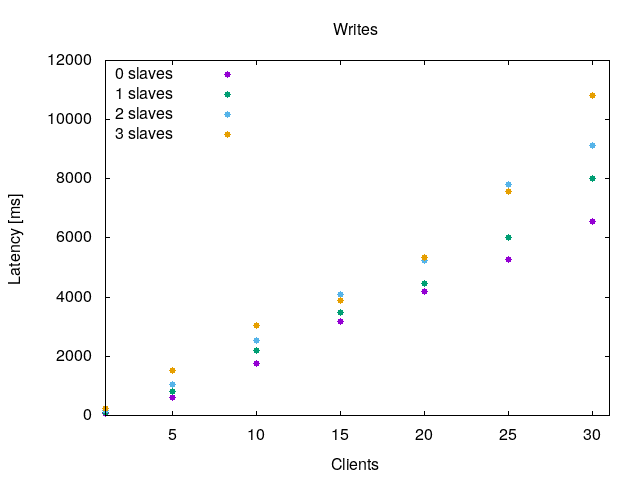
\includegraphics[width=0.9\textwidth]{images/writes.png}
    \caption{Escritas}
    \label{fig:w}
\end{figure}

\begin{figure}
    \centering
    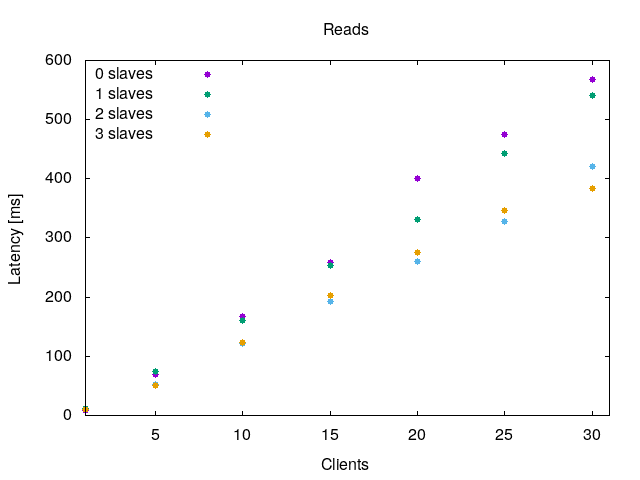
\includegraphics[width=0.9\textwidth]{images/reads.png}
    \caption{Leituras}
    \label{fig:r}
\end{figure}


%Através das tabelas \ref{fig:write_slaves0} a \ref{fig:read_slaves3}, é possível observar o impacto que o PGpool tem nos vários tipos de \textit{queries}. 

Para \textit{queries} de escrita não se verifica melhorias (piora até com o aumento do número de \textit{slaves}), isto porque o PGpool não tem nenhum mecanismo de balanceamento para \textit{queries} deste tipo visto que estas transacções têm sempre de chegar a todos as réplicas.

Já para \textit{queries} de leitura são visíveis as melhorias na latência média dos pedidos, visto que para este tipo de pedidos o PGpool faz balanceamento de carga dividindo os pedidos pelas várias réplicas. 

Num cenário com apenas um cliente a latência média piora quando são utilizados múltiplos \textit{slaves}, isto acontece uma vez que os pedidos estarão a passar pelo PGpool tendo assim um \textit{overhead} adicional. 
Ao comparar os casos de um \textit{cluster} com 3 \textit{slaves} e um com 2 \textit{slaves} (Figura \ref{fig:r}), concluí-se que a latência média só melhora com 30 clientes, verificando que o aumento de réplicas só compensa aumentando também o \textit{workload}.



\subsection{Conclusão}
Com os resultados obtidos podemos verificar que para um \textit{cluster} de base de dados, usando o PGpool, o paralelismo obtido para vários clientes concorrentes melhora a latência média das transacções de leitura, verificando que até certo ponto o impacto do \textit{cluster} com o aumento do número de réplicas só melhora a latência para um aumento do \textit{workload}. Esta situação foi verificada para o caso em que a latência de um \textit{cluster} com 3 réplicas só melhorou quando o número de clientes atingiu os 30, sendo pior para os outros casos. \\

O uso do sistema PGpool melhora apenas a latência média das transacções de leitura, piorando significativamente as transacções de escrita. 

Assim, a instalação do PGpool num \textit{cluster} de base de dados só será benéfica caso este seja alvo, maioritariamente, de transacções de leitura, caso contrário deverá ser dada atenção ao deterioramento da performance das transacções de escrita, tentando procurar soluções para mitigar este problema.

\section{Parte 2}

\subsection{Introdução}
Nesta segunda parte o PgPool foi analisado em instâncias no aws. Devido a dificuldades técnicas não foi possível correr de forma distribuída em vários nós, ainda assim é possível analisar a \textit{performance} em diferentes instâncias com diferentes recursos e retirar de que modo estes afetam o PgPool. Para tentar simular a distribuição entre várias instâncias foi limitada a utilização do CPU para 10\% para os vários containers, esta abordagem tem várias desvantagens em relação à análise distribuída sendo a principal o facto de se ignorar a latência da rede.

\subsection{Características das Maquinas}

Quatro maquinas diferentes foram utilizadas para realizar as experiências, todas estas a correr linux (kernel 4.15.0-1051-aws).

\begin{table}
    \centering
    \begin{tabular}{||c|c|c||}
        \hline
         Maquina & CPU & Disco \\\hline
         1 & Intel Xeon E5-2686 v4 octa-core 2.3GHz & EBS, General Purpose SSD \\\hline
         2 & Intel Xeon E5-2686 v4 octa-core 2.3GHz & EBS, Magnetic (standard) \\\hline
         3 & Intel Xeon E5-2676 v3 dual-core 2.4GHz & EBS, General Purpose SSD \\\hline
         4 & Intel Xeon E5-2676 v3 dual-core 2.4GHz & EBS, Magnetic (standard) \\\hline
    \end{tabular}
    \label{tab:maquinas}
    \caption{Maquinas utilizadas}
\end{table}

\subsection{Workload}

O \textit{workload} utilizado para as benchmarks foi o seguinte~\cite{pgbench}:
\subsubsection{Escritas}
\begin{minted}{sql}
BEGIN;
UPDATE pgbench_accounts SET abalance = abalance + :delta 
    WHERE aid = :aid;
    
SELECT abalance FROM pgbench_accounts 
    WHERE aid = :aid;
    
UPDATE pgbench_tellers SET tbalance = tbalance + :delta 
    WHERE tid = :tid;
    
UPDATE pgbench_branches SET bbalance = bbalance + :delta 
    WHERE bid = :bid;
    
INSERT INTO pgbench_history (tid, bid, aid, delta, mtime)
    VALUES (:tid, :bid, :aid, :delta, CURRENT_TIMESTAMP);
    
END;
\end{minted}

\subsubsection{Leituras}
\begin{minted}{sql}
BEGIN;
SELECT abalance FROM pgbench_accounts 
    WHERE aid = :aid;
END;
\end{minted}

Estes \textit{workloads} são repetidos durante 60 segundos tentando realizar o máximo de transacções possíveis.




\subsection{Benchmark}
\subsubsection{Parâmetros}
Iram ser analisados 5 parâmetros do sistema com dois níveis cada um. Dois parâmetros são intrínsecos ao PgPool enquanto os outros 3 serão recursos das instâncias em que o sistema irá ser analisado.\newline
Parâmetros intrínsecos ao sistema:
\begin{itemize}
    \item A - Número de nós (2/5)
    \item D - Connection cache (On / Off)
\end{itemize}
Parâmetros das máquinas:
\begin{itemize}
    \item B - CPU Cores (2/8)
    \item C - Disco (HDD/SSD)
    \item E - Ram (521Mb / 1Gb)
\end{itemize}

Fazer um benchmark completo tendo 5 factores com 2 níveis cada implica realizar um total de $2^5=32$ experiências. Para simplificar e facilitar a análise reduziu-se o número de experiências para $2^{(5-2)}=8$. De modo a reduzir o número de experiências 2 dos 5 parâmetros vão ser definidos como combinação de outros dois parâmetros da seguinte da maneira:\newline

\begin{table}
    \centering
    \begin{tabular}{|| c | c | c | c | c | c ||} 
         \hline
          Experiência & A & B & C & D $(A.B)$ & E $(B.C)$ \\ [0.5ex] 
         \hline\hline
         1 & -1 & -1 & -1 & 1 & 1\\ 
         \hline
         2 & -1 & -1 & 1 & 1 & -1\\ 
         \hline
         3 & -1 & 1 & -1 & -1 & -1\\ 
         \hline
         4 & -1 & 1 & 1 & -1 & 1\\ 
         \hline
         5 & 1 & -1 & -1 & -1 & 1\\ 
         \hline
         6 & 1 & -1 & 1 & -1 & -1\\ 
         \hline
         7 & 1 & 1 & -1 & 1 & -1\\ 
         \hline
         8 & 1 & 1 & 1 & 1 & 1\\ 
        \hline
    \end{tabular}
    \caption{Sign tables}
\end{table}

\subsubsection{Métricas:}
A métricas medidas foram as mesmas analisadas na primeira parte, latência de operações de escrita e leitura. Na primeira parte do projeto chegamos a conclusão dos factores que influenciam positivamente e negativamente a escalabilidade do sistema.\newline
Para operações de leitura a latência melhorava com mais nós e para operações de escrita a latência piorava bastante em relação ao benefícios que o sistema trazia para operações de leitura. Assim o PgPool apenas era benéfico se o sistema realizasse maioritariamente operações de leitura a não ser que fosse possível mitigar o aumento da latência de operações de escrita com o aumento do número de nós, foi possível nesta parte analisar e quantificar de que forma era possível mitigar este problema.

\subsubsection{Resultados:}
\begin{table}
    \centering
    \begin{tabular}{|| c | c | c | c | c | c | c | c ||} 
         \hline
         Experiência & Nós & CPU Cores & Disco & Connection Cache & Ram & Leituras[ms] & Escritas[ms]\\ [0.5ex] 
         \hline\hline
         1 & 2 & 2 & HDD & ON & 1GB & 45.80 & 1273.01\\ 
         \hline
         2 & 2 & 2 & SSD & ON & 512Mb & 44.43 & 842.77\\ 
         \hline
         3 & 2 & 8 & HDD & OFF & 512Mb & 10.815 & 1248.694\\ 
         \hline
         4 & 2 & 8 & SSD & OFF & 1GB & 9.878 & 695.192\\ 
         \hline
         5 & 5 & 2 & HDD & OFF & 1GB & 48.039 & 3218.947\\ 
         \hline
         6 & 5 & 2 & SSD & OFF & 512Mb & 45.447 & 1615.756\\ 
         \hline
         7 & 5 & 8 & HDD & ON & 512Mb & 11.293 & 2156.891\\ 
         \hline
         8 & 5 & 8 & SSD & ON & 1GB & 24.687 & 1534.96\\ 
         \hline
    \end{tabular}
    \caption{Resultados - Latência}
\end{table}
Com base nos resultados foi determinado o impacto de cada parâmetro em análise tanto para as operações de escritas como para operações de leitura.

\begin{itemize}
    \item q0: performance base
    \item qA: performance associada ao número de nós
    \item qB: performance associada aos cores utilizados
    \item qC: performance associada ao tipo de disco
    \item qD: performance associada ao parâmetro de \textit{connection cache}
    \item qE: performance associada à RAM
\end{itemize}

\subsubsection{Leituras:}
\noindent Cálculo do peso das \textit{performances} para operações de leitura:
\begin{itemize}
    \item q0: 30.048
    \item qA: -2.317
    \item qB: \textcolor{red}{15.880}
    \item qC: -1.061
    \item qD: 1.503
    \item qE: 2.052
\end{itemize}
Variação total da latência: 
\begin{equation}
    SS_{T}= 8*(qA^2+qB^2+qC^2+qD^2+qE^2)=2121.28
\end{equation}

Efeito em percentagem de cada parâmetro no sistema:
\begin{itemize}
    \item Nós (qA): 2.2\%
    \item CPU Cores (qB): \textcolor{red}{95.12\%}
    \item Disco (qC): 0.43\%
    \item Connection cache (qD): 0.85\%
    \item RAM (qE): 1.50\%
\end{itemize}

\subsubsection{Escritas:}
Cálculo do peso das \textit{performances} para operações de escrita:
\begin{itemize}
    \item q0: 1573.277
    \item qA: \textcolor{red}{-558.361}
    \item qB: 164.343
    \item qC: \textcolor{red}{401.108}
    \item qD: -121.369
    \item qE: 107.249
\end{itemize}
Variação total da latência: 
\begin{equation}
    SS_{T}= 8*(qA^2+qB^2+qC^2+qD^2+qE^2)=4207171.70
\end{equation}

Efeito em percentagem de cada parâmetro no sistema:
\begin{itemize}
    \item Nós (qA): \textcolor{red}{59.28\%}
    \item CPU Cores (qB): 5.14\%
    \item Disco (qC): \textcolor{red}{30.59\%}
    \item Connection cache (qD): 2.8\%
    \item RAM (qE): 2.19\%
\end{itemize}

\subsection{Conclusões}
Como visto já na parte 1 o comportamento do sistema varia bastante conforme a natureza do \textit{workload}, consequentemente o impacto dos vários parâmetros também é diferente para vários tipos de workload. No geral parâmetros como o \textit{connection cache} e RAM não tiveram grande impacto, este facto pode ser explicado pelo facto de o workload usado não ser suficientemente grande para beneficiar destes parâmetros.

\subsubsection{Leituras:}
Para operações de leitura o parâmetro que mais afeta a \textit{performance}, positivamente, é o poder de processamento (número de cores), tendo um impacto de 95\%. Isto pode ser explicado pelo facto de o número de cores, tal como o número de nós, aumentar o nível de paralelismo do sistema.

\subsubsection{Escritas:}
Para operações de escrita o parâmetro que mais afetou negativamente o sistema foi o número de nós, tal como explicado já na parte 1 o facto de nas escritas todos os nós terem que estar consistentes para correr as operações seguintes piora a performance do sistema em 59.2\%. O tipo de disco foi o segundo parâmetro que afetou mais o sistema positivamente, tendo um impacto de 30.59\% na performance. Este comportamento é esperado devido ao facto de a velocidade de leituras/escritas do disco afetar a velocidade de cada transação.

%
% ---- Bibliography ----
%
% BibTeX users should specify bibliography style 'splncs04'.
% References will then be sorted and formatted in the correct style.
%
% \bibliographystyle{splncs04}
% \bibliography{mybibliography}
%
\bibliography{bibliography.bib}
\bibliographystyle{unsrt}
\end{document}